%!TEX encoding = UTF-8 Unicode
%!TEX root = ../lect-w12.tex

%%%



\Subsection{Veckans labb: \texttt{survey}}
\begin{Slide}{Veckans labb: \texttt{survey}}\SlideFontTiny
\begin{minipage}{0.71\textwidth}
\vspace{0.25em}
\Emph{Förberedelse:}
\begin{itemize}
\item Studera givna koden: {\SlideFontTiny \href{https://github.com/lunduniversity/introprog/tree/master/workspace/w12_survey/src/main/scala/stats}{workspace/w12\_survey}}
\item Fyll i denna enkät:
\\{\SlideFontTiny \url{https://goo.gl/forms/hC6JK2UQXVpbGECc2}}
\item Se svar från 2016: \url{http://cs.lth.se/pgk/favorit}
\end{itemize}

\Emph{Grunduppgift:}
\begin{itemize}
\item Klassen \code{Table} för hantering av strängmatriser med rubrikrad från kolumnsepararade textfiler.
\item Öva på att kombinera matriser, sortering, registrering för att räkna statistik.
\item Använda inbyggda sorteringsfunktioner: \\\code{sortBy} och \code{sortWith}
\item Implementera din egen sortering ''från scratch''.
\end{itemize}
\Emph{Extrauppgift:}
\begin{itemize}
\item Implementera stapeldiagram.
\end{itemize}
\end{minipage}
\hfill\begin{minipage}{0.25\textwidth}
\centering
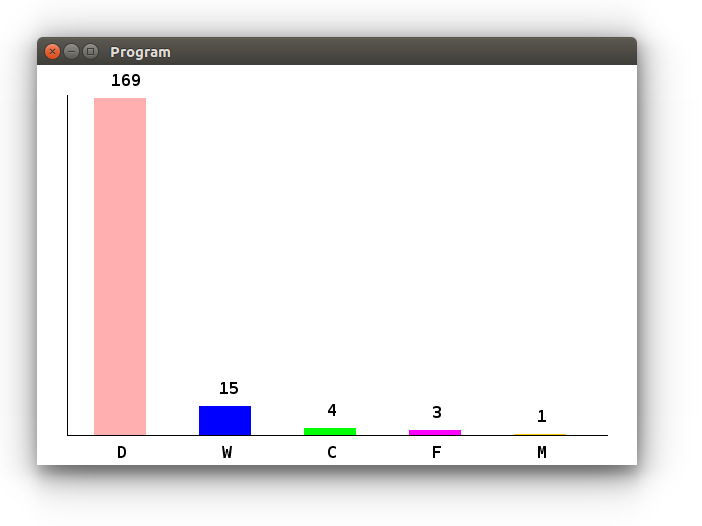
\includegraphics[width=0.9\textwidth]{../img/survey/bar}

\vspace{2em}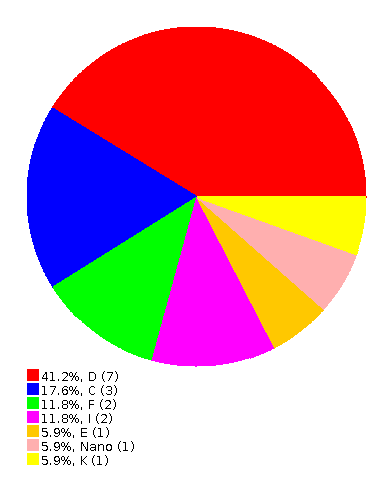
\includegraphics[width=0.7\textwidth]{../img/survey/pie}
\end{minipage}
\end{Slide}
